\documentclass[border=8pt]{standalone}
\usepackage{tikz}
\usetikzlibrary{positioning,arrows.meta,fit,backgrounds,calc}
\begin{document}
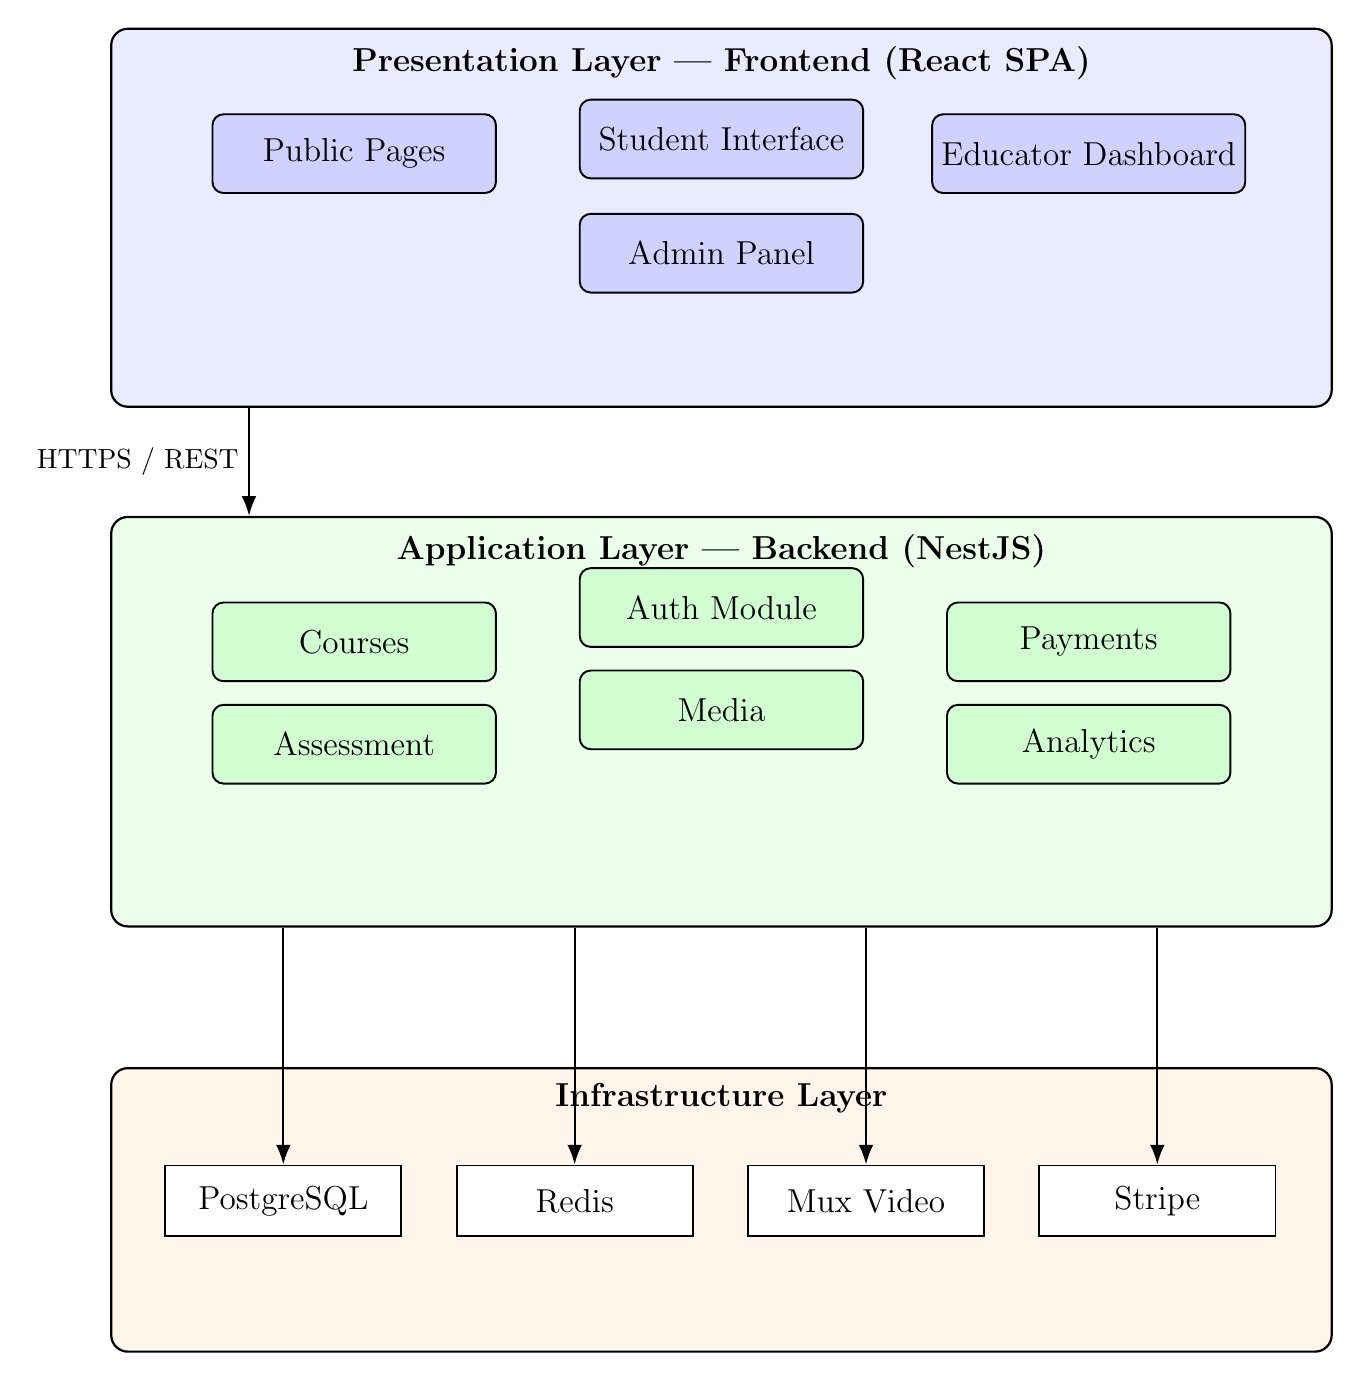
\begin{tikzpicture}[
  font=\large,
  layer/.style={rounded corners=6pt, draw=black, line width=0.8pt, minimum width=15.5cm, align=center},
  title/.style={font=\bfseries\large},
  block/.style={rounded corners=4pt, draw=black, line width=0.7pt, minimum width=3.6cm, minimum height=1cm, align=center, fill=white},
  infra/.style={draw=black, line width=0.7pt, minimum width=3cm, minimum height=0.9cm, align=center, fill=white},
  arr/.style={-{Latex[length=2.5mm]}, line width=0.8pt}
]

% ---------- Presentation Layer ----------
\node[layer, minimum height=4.8cm, fill=blue!8] (pres) at (0,9) {};
\node[title] (prestitle) at ($(pres.north)+(0,-0.45)$) {Presentation Layer --- Frontend (React SPA)};

\node[block, fill=blue!18] (public)   at ($(pres.north west)+(3.1,-1.6)$) {Public Pages};
\node[block, fill=blue!18] (student)  at ($(pres)+(0,1.0)$)               {Student Interface};
\node[block, fill=blue!18] (educator) at ($(pres.north east)+(-3.1,-1.6)$) {Educator Dashboard};
\node[block, fill=blue!18] (admin)    at ($(pres)+(0,-0.45)$)            {Admin Panel};

% ---------- Application Layer ----------
\node[layer, minimum height=5.2cm, fill=green!8] (app) at (0,2.6) {};
\node[title] (apptitle) at ($(app.north)+(0,-0.45)$) {Application Layer --- Backend (NestJS)};

\node[block, fill=green!18] (courses)    at ($(app.north west)+(3.1,-1.6)$) {Courses};
\node[block, fill=green!18] (authmod)    at ($(app)+(0,1.45)$)              {Auth Module};
\node[block, fill=green!18] (payments)   at ($(app.north east)+(-3.1,-1.6)$) {Payments};
\node[block, fill=green!18] (assessment) at ($(courses)+(0,-1.3)$)          {Assessment};
\node[block, fill=green!18] (media)      at ($(authmod)+(0,-1.3)$)          {Media};
\node[block, fill=green!18] (analytics)  at ($(payments)+(0,-1.3)$)         {Analytics};

% connector pres -> app : routed at a fixed x offset, clear of the centred title text
\draw[arr] ($(pres.south)+(-6.0,0)$) -- node[left, font=\normalsize] {HTTPS / REST} ($(app.north)+(-6.0,0)$);

% ---------- Infrastructure Layer ----------
\node[layer, minimum height=3.6cm, fill=orange!8] (infraLayer) at (0,-3.6) {};
\node[title] (infratitle) at ($(infraLayer.north)+(0,-0.4)$) {Infrastructure Layer};

\node[infra] (pg)     at ($(infraLayer.north west)+(2.2,-1.7)$) {PostgreSQL};
\node[infra] (redis)  at ($(pg)+(3.7,0)$)                       {Redis};
\node[infra] (mux)    at ($(redis)+(3.7,0)$)                    {Mux Video};
\node[infra] (stripe) at ($(mux)+(3.7,0)$)                      {Stripe};

% Exit the application layer at the SAME x as each infra target (not from the
% individual module's south side) so the four lines never cross one another
% or pass over a sibling module's label.
\draw[arr] (app.south -| pg)     -- (pg.north);
\draw[arr] (app.south -| redis)  -- (redis.north);
\draw[arr] (app.south -| mux)    -- (mux.north);
\draw[arr] (app.south -| stripe) -- (stripe.north);

\end{tikzpicture}
\end{document}
